\langsection[subsection]{Increasing Conspicuity}{Повышение заметности}





\begin{langblock}{0.425}
	\begin{eng}
	
	In crashes with motorcyclists, drivers often say that they never saw the motorcycle. From ahead or behind, a motorcycle's outline is much smaller than a car's. Also, it's hard to see something you are not looking for, and most drivers are not looking for motorcycles. More likely, they are looking through the skinny, two- wheeled silhouette in search of cars that may pose a problem to them.
	
	Even if a driver does see you coming, you aren't necessarily safe.  Smaller vehicles appear farther away, and seem to be traveling slower than they actually are. It is common for drivers to pull out in front of motorcyclists, thinking they have plenty of time. Too often, they are wrong.
	
	However, you can do many things to make it easier for others to recognize you and your cycle.
	\end{eng}
	\begin{rus}
		
		В ДТП с участием мотоциклистов водители часто говорят, что вообще не видели мотоцикл. Как спереди, так и сзади силуэт мотоцикла гораздо уже, чем у автомобиля. Кроме того, автомобилисты замечают лишь то, что ищут, а мотоциклы в этот набор не входят: их взгляд, минуя узкий силуэт мотоцикла, скользит дальше в поисках других автомобилей "--- именно тех, кто могут представлять для них опасность.
		
		Даже если водитель и заметит вас, это не означает, что вы в безопасности. Небольшие транспортные средства кажутся более отдаленными и двигающимися медленнее, чем на самом деле. Водители часто выезжают перед мотоциклистами, полагая, что у них достаточно времени. И они слишком часто ошибаются.
		
		Однако вы можете принять ряд мер, чтобы было легче заметить Вас и ваш мотоцикл.
\end{rus}
\end{langblock}


\langsection[subsubsection]{Clothing}{Одежда}



\begin{langblock}{0.425}
	\begin{eng}
	
	Most crashes occur in broad daylight. Wear bright colored clothing to increase your chances of being seen. Remember, your body is half of the visible surface area of the rider/motorcycle unit.
	
	Bright orange, red, yellow or green jackets or vests are your best bets for being seen. Your helmet can do more than protect you in a crash.  Brightly colored helmets can also help others see you.
	
	Any bright color is better than drab or dark colors. Reflective, bright colored clothing (helmet and jacket or vest) is best.
	
	Reflective material on a vest and on the sides of the helmet will help drivers coming from the side spot you.  Reflective material can also be a big help for drivers coming toward you or from behind.
	\end{eng}
	\begin{rus}
		
		Большинство ДТП происходит при дневном свете. Носите одежду ярких цветов, чтобы быть более заметным. Помните: ваше тело это половина видимого силуэта мотоцикла.
		
		Ярко-оранжевые, красные, желтые или зеленые куртки или жилеты "--- лучший выбор, чтобы вас заметили. Шлем может не только защитить вас при аварии. Яркие шлемы также делают вас более заметным для других участников дорожного движения.
		
		Любой яркий цвет лучше, чем тусклые или темные оттенки. Лучше выбор "--- светоотражающая одежда ярких цветов (шлем и куртка или жилет).
		
		Светоотражающий материал на жилете и по бокам шлема поможет водителям заметить вас при приближении сбоку. Светоотражающий материал также поможет водителям вас заметить как спереди так и сзади\footnote{Тут скорее всего имеется ввиду не Reflective, а Retroreflective -- световозвращающие материалы. Когда отражение идет в сторону источника света. Все современные вставки на одежде именно Retroreflective}.
\end{rus}
\end{langblock}



\langsection[subsubsection]{Headlight}{Фара}



\begin{langblock}{0.425}
	\begin{eng}
	
	Motorcycles manufactured during or after 1973 are required by law to use headlights at all times. The headlight is the best way to help others see you. Studies show that during the day, a motorcycle with its light on is twice as likely to be noticed.
	\end{eng}
	\begin{rus}
		
		По закону, на мотоциклах, выпущенных начиная с 1973 года, фары должны быть включены днем и ночью. Фары "--- это лучший способ стать заметным для других участникам движения. Исследования показывают, что мотоцикл с включенными днем фарами заметнее в два раза.
\end{rus}
\end{langblock}



\langsection[subsubsection]{Signals}{Поворотники}


\begin{figure}[htbp]
	\centering
	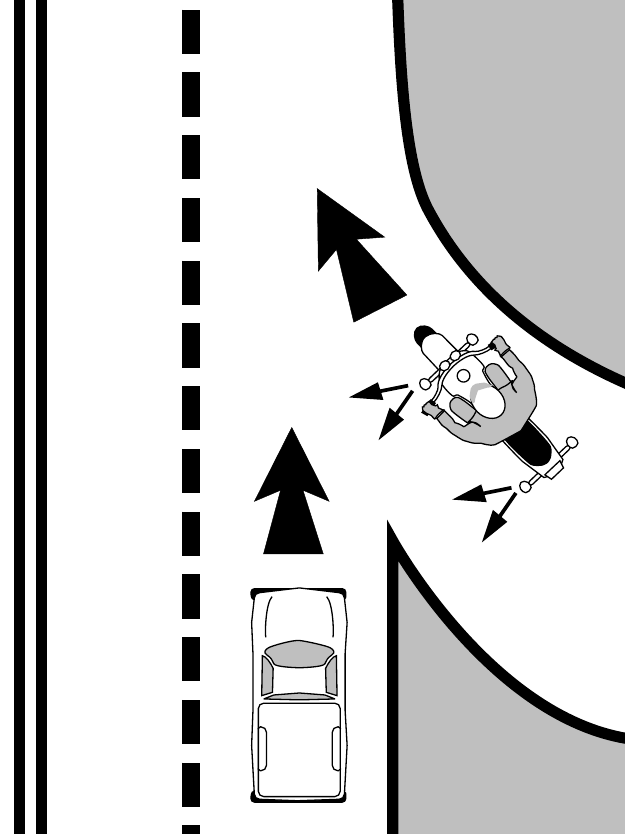
\includegraphics[width=0.45\textwidth, frame]{images/signaling.png}
	\caption{Signaling}
	\label{fig:signaling}
\end{figure}



\begin{langblock}{0.425}
	\begin{eng}
	
	The signals on a motorcycle are similar to those on a car. They tell others what you plan to do. However, due to a rider's added vulnerability, signals are even more important. Use them anytime you plan to change lanes or turn. Use them even when you think no one else is around. It's the car you don't see that's going to give you the most trouble. Your signal lights also make you easier to spot.  That's why it's a good idea to use your turn signals even when what you plan to do is obvious.
	
	When you enter a freeway, drivers approaching from behind are more likely to see your signal blinking and make room for you.
	
	Turning your signal light on before each turn reduces confusion and frustration for the traffic around you. Once you turn, make sure your signal is off or a driver may pull directly into your path, thinking you plan to turn again. Use your signals at every turn so drivers can react accordingly. Don't make them guess what you intend to do.
	\end{eng}
	\begin{rus}
		
		Сигналы на мотоцикле аналогичны сигналам на автомобиле. Они сообщают окружающим о ваших намерениях. Однако из-за большей уязвимости мотоциклиста сигналы приобретают еще большее значение. Используйте их всякий раз, когда собираетесь сменить полосу движения или повернуть. Используйте их даже тогда, когда вам кажется, что поблизости никого нет. Автомобиль которого вы не заметили источник наибольшей опасности. Поворотники также делают вас более заметным.  Вот почему надо включать поворотники даже в тех случаях, когда ваши намерения очевидны.
		
		Когда вы выезжаете на автомагистраль, водители с большей вероятностью заметят мигающий поворотник и уступят вам правую полосу.
		
		Включение поворотника перед каждым поворотом снижает путаницу и раздражение у окружающих. После поворота убедитесь, что поворотник \textbf{ВЫКЛ}ючен, иначе водитель может поехать прямо на вас, полагая, что вы собираетесь поворачивать. Используйте поворотники при каждом повороте, чтобы водители могли соответствующим образом реагировать. Не вынуждайте их гадать о ваших намерениях.
\end{rus}
\end{langblock}


\langsection[subsubsection]{Brake Light}{Стоп-сигнал}


\begin{langblock}{0.425}
	\begin{eng}
	
	Your motorcycle's brake light is usually not as noticeable as the brake lights on a car -- particularly when your taillight is on. (The tail light goes on with the headlight.) If the situation will permit, help others notice you by flashing your brake light before you slow down. It is especially important to flash your brakelight before:
	\begin{description} [noitemsep]
	\item [You slow more quickly] than others might expect (turning off a high- speed highway).
	\item [You slow where] others may not expect it (in the middle of a block or at an alley).
	\end{description}
		
	If you are being followed closely, it's a good idea to flash your brake light before you slow. The tailgater may be watching you and not see something ahead that will make you slow down. This will hopefully discourage them from tailgating and warn them of hazards ahead they may not see.
	\end{eng}
	\begin{rus}
		Стоп-сигнал мотоцикла, как правило, менее заметен, чем стоп-сигналы автомобиля "--- особенно когда горит задний габаритный огонь. (Задний габаритный огонь включается вместе с фарой) Если позволяет ситуация, для большей заметности, помигайте стоп-сигналом перед тем, как начать торможение. Особенно важно моргать стоп-сигналом перед тем, как:
		
		\begin{description} [noitemsep]
			\item [Вы замедляетесь] агрессивнее, чем могут ожидать окружающие (например, при съезде с скоростной автомагистрали).
			\item [Вы замедляетесь] там, где другие этого не ожидают (в середине квартала или в переулке).
		\end{description}
		
		Если за вами едут слишком близко, рекомендуется мигать стоп-сигналом перед замедлением. Водитель, едущий слишком близко сзади, может смотреть на вас, а не на то что  впереди вас, и пропустить то, что заставит вас замедлиться. Это так же может отвадить его висеть у вас на хвосте и предупредит о возможных опасностях впереди.
\end{rus}
\end{langblock}



\langsection[subsubsection]{Using Your Mirrors}{Зеркала}


\begin{figure}[htbp]
	\centering
	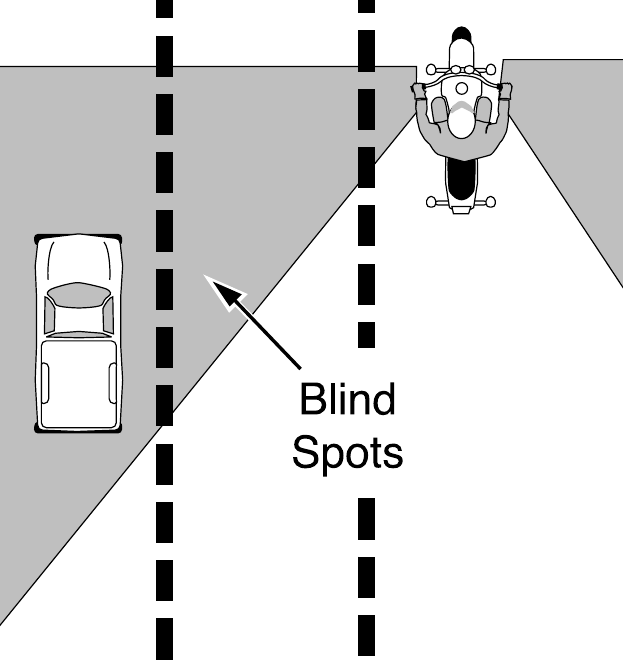
\includegraphics[width=0.45\textwidth, frame]{images/using_mirrors.png}
	\caption{Using mirrors}
	\label{fig:using_mirrors}
\end{figure}



\begin{langblock}{0.425}
	\begin{eng}
	
	While it's most important to keep track of what's happening ahead, you can't afford to ignore situations behind. Traffic conditions change quickly. Knowing what's going on behind is essential for you to make a safe decision about how to handle trouble ahead.
	
	Frequent mirror checks should be part of your normal searching routine.  Make a special point of using your mirrors:
	
	\begin{description} [noitemsep]
		\item [When you are stopped] at an intersection. Watch cars coming up from behind. If the driver isn't paying attention, he could be on top of you before he sees you.
		\item [Before you change lanes.] Make sure no one is about to pass you.
		\item [Before you slow down.] The driver behind may not expect you to slow, or may be unsure about where you will slow. For example, you signal a turn and the driver thinks you plan to turn at a distant intersection, rather than at a nearer driveway.
	\end{description}
	
	Some motorcycles have rounded (convex) mirrors. These provide a wider view of the road behind than do flat mirrors. They also make cars seem farther away than they really are. If you are not used to convex mirrors, get familiar with them. 
	
	(While you are stopped, pick out a parked car in your mirror. Form a mental image of how far away it is. Then, turn around and look at it to see how close you came.)
	
	Practice with your mirrors until you become a good judge of distance.  Even then, allow extra distance before you change lanes.
	\end{eng}
	\begin{rus}
		
		И хотя самое главное это то, что происходит впереди, нельзя игнорировать ситуацию и сзади. Обстановка на дороге меняется быстро. Знание того, что происходит сзади, крайне важно для принятия правильного решения проблемы возникшей спереди.
		
		Частые проверки зеркал должны стать частью вашей обычной практики обзора. Особое внимание уделяйте использованию зеркал:
		
		\begin{description} [noitemsep]
			\item [Когда вы остановились] на перекрестке, следите за автомобилями сзади. Если водитель невнимателен, то он переедет вас, прежде чем заметит.
			\item [Перед сменой полосы] убедитесь, что никто не собирается вас обгонять.
			\item [Перед тем как снизить скорость.] Водитель сзади может не ожидать вашего торможения в принципе или в данный момент. Например, вы включаете поворотник, и водитель думает, что вы собираетесь повернуть на ближайшем перекрестке, тогда как вы съезжаете в во двор.
		\end{description}
		
		Некоторые мотоциклы оснащены сферическими зеркалами (выпуклые). Они обеспечивают более широкий обзор дороги сзади, чем плоские зеркала. Однако, в них предметы кажутся более отдаленными, чем на самом деле. Если вы не привыкли к выпуклым зеркалам, попрактикуйтесь в их использовании.
		
		(Во время остановки выберите в зеркале припаркованный автомобиль. Представьте себе, на каком расстоянии он находится. Затем обернитесь и посмотрите на него, чтобы оценить, насколько близко он на самом деле.)
		
		Потренируйтесь с зеркалами, пока не научитесь точно оценивать расстояние.  Даже после этого оставляйте дополнительный запас на всякий случай.
\end{rus}
\end{langblock}





\langsection[subsubsection]{Head Checks}{Поворот головы}


\begin{langblock}{0.425}
	\begin{eng}
	
	Checking your mirrors is not enough. Motorcycles have "blind spots" like cars. Before you change lanes, turn your head, and look to the side for other vehicles.
	
	On a road with several lanes, check the far lane and the one next to you. A driver in the distant lane may head for the same space you plan to take.
	
	Frequent head checks should be your normal scanning routine, also.  Only by knowing what is happening all around you, are you fully prepared to deal with it.
	\end{eng}
	\begin{rus}
		
		Одного взгляда в зеркала недостаточно. У мотоциклов, как и у автомобилей, есть «слепые зоны». После взгляда в зеркало, но перед сменой полосы поверните голову и посмотрите в сторону. Убедитесь в отсутствии других транспортных средств.
		
		На многополосной дороге проверяйте не только полосу, в которую перестраиваетесь, но и следующую за ней: водитель в дальней полосе может направляться в то же самое место, что и вы.
		
		Частые взгляды по сторонам также должны стать вашей обычной практикой.  Только зная, что происходит вокруг, вы будете полностью готовы к любой ситуации.
\end{rus}
\end{langblock}

\langsection[subsubsection]{Horn}{Клаксон}


\begin{langblock}{0.425}
	\begin{eng}
	
	Be ready to use your horn to get someone's attention quickly.  It is a good idea to give a quick beep before passing anyone that may move into your lane.
	
	Here are some situations:
	
	\begin{description} [noitemsep]
		\item [A driver] in the lane next to you is driving too closely to the vehicle ahead and may want to pass.
		\item [A parked car] has someone in the driver's seat.
		\item [Someone] is in the street, riding a bicycle or walking.
	\end{description}
	
	In an emergency, press the horn button loud and long. Be ready to stop or swerve away from the danger.
	
	Keep in mind that a motorcycle's horn isn't as loud as a car's, therefore, use it, but don't rely on it.  Other strategies, like having time and space to maneuver, may be appropriate along with the horn.
	\end{eng}
	\begin{rus}
		
		Держи клаксон наготове, чтобы быстро привлечь внимание окружающих. Дайте упреждающий короткий сигнал перед тем, как обгонять кого-либо.
		
		Вот несколько типичных ситуаций:
		
		\begin{description} [noitemsep]
			\item [Водитель] на соседней полосе едет слишком близко к впереди идущему транспортному средству и, возможно, собирается его обогнать.
			\item [В припаркованном] автомобиле кто-то сидит на месте водителя.
			\item [По улице] кто-то едет на велосипеде или идет пешком.
		\end{description}
		
		В экстренной ситуации жмите клаксон без колебаний (громкий и продолжительный сигнал). Будьте готовы остановиться или маневрировать.
		
		Помните, что звуковой сигнал мотоцикла не такой громкий, как у автомобиля, используйте его, но не полагайтесь на него полностью. Наряду с сигналом держите запас времени и дистанции для маневра.
\end{rus}
\end{langblock}


\langsection[subsubsection]{Riding at Night}{Езда по ночам}



\begin{langblock}{0.425}
	\begin{eng}
	
	At night it is harder for you to see and be seen. Picking your headlight or taillight out of the car lights around you is not easy for other drivers. To compensate, you should:
	
	\begin{description} [noitemsep]
		\item[Reduce Your Speed] Ride even slower than you would during the day -- particularly on roads you don't know well. This will increase your chances of avoiding a hazard.
		\item[Increase Distance] Distances are harder to judge at night than during the day. Your eyes rely upon shadows and light contrasts to determine how far away an object is and how fast it is coming. These contrasts are missing or distorted under artificial lights at night. Open up a three-second following distance or more. And allow more distance to pass and be passed.
		\item[Use the Car Ahead] The headlights of the car ahead can give you a better view of the road than even your high beam can. Taillights bouncing up and down can alert you to bumps or rough pavement.
		\item[Use Your High Beam] Get all the light you can. Use your high beam whenever you are not following or meeting a car. Be visible, wear reflective materials when riding at night.
		\item[Be flexible] about lane position Change to whatever portion of the lane is best able to help you see, be seen, and keep an adequate space cushion.
	\end{description}
	\end{eng}
	\begin{rus}
		
		Ночью сложнее самому видеть и быть заметным для других. В свете фар и фонарей, фары и задний габарит мотоцикла не так заметены как фары или задние фонари автомобиля. Чтобы это компенсировать, вам следует:
		
		\begin{description} [noitemsep]
			\item [Снизить скорость] Езжайте еще медленнее, чем днем "--- особенно на незнакомых дорогах. Это увеличит ваши шансы избежать неприятностей.
			\item [Увеличьте дистанцию] Ночью сложнее оценить расстояния, чем днем. Ваши глаза полагаются на тени и контрасты света, чтобы определить, на каком расстоянии находится объект и с какой скоростью он приближается. При искусственном освещении ночью эти контрасты отсутствуют или искажаются. Соблюдайте дистанцию в три секунды или более. Также оставляйте больше места, когда обгоняете сами и обгоняют вас.
			\item [Ориентируйтесь] на впереди идущий автомобиль. Фары впереди идущего автомобиля могут обеспечить вам обзор и освещение дороги даже лучше, чем ваш дальний свет. Прыгающие вверх-вниз задние фонари могут предупредить вас о неровностях или плохом состоянии дорожного покрытия.
			\item[Используйте дальний свет] Обеспечьте себе максимальное освещение. Включайте дальний свет, когда вы не едете в колонне и нет встречного транспорта. Будьте заметны: носите светоотражающие элементы при езде ночью.
			\item [Будьте гибкими] в выборе положения на полосе движения. Переместитесь в ту часть полосы, которая дает лучше обзор, позволяет быть заметным и сохранять достаточную дистанцию и интервал.
		\end{description}
\end{rus}
\end{langblock}









